% Created by tikzDevice version 0.12.3.1 on 2021-07-01 11:40:12
% !TEX encoding = UTF-8 Unicode
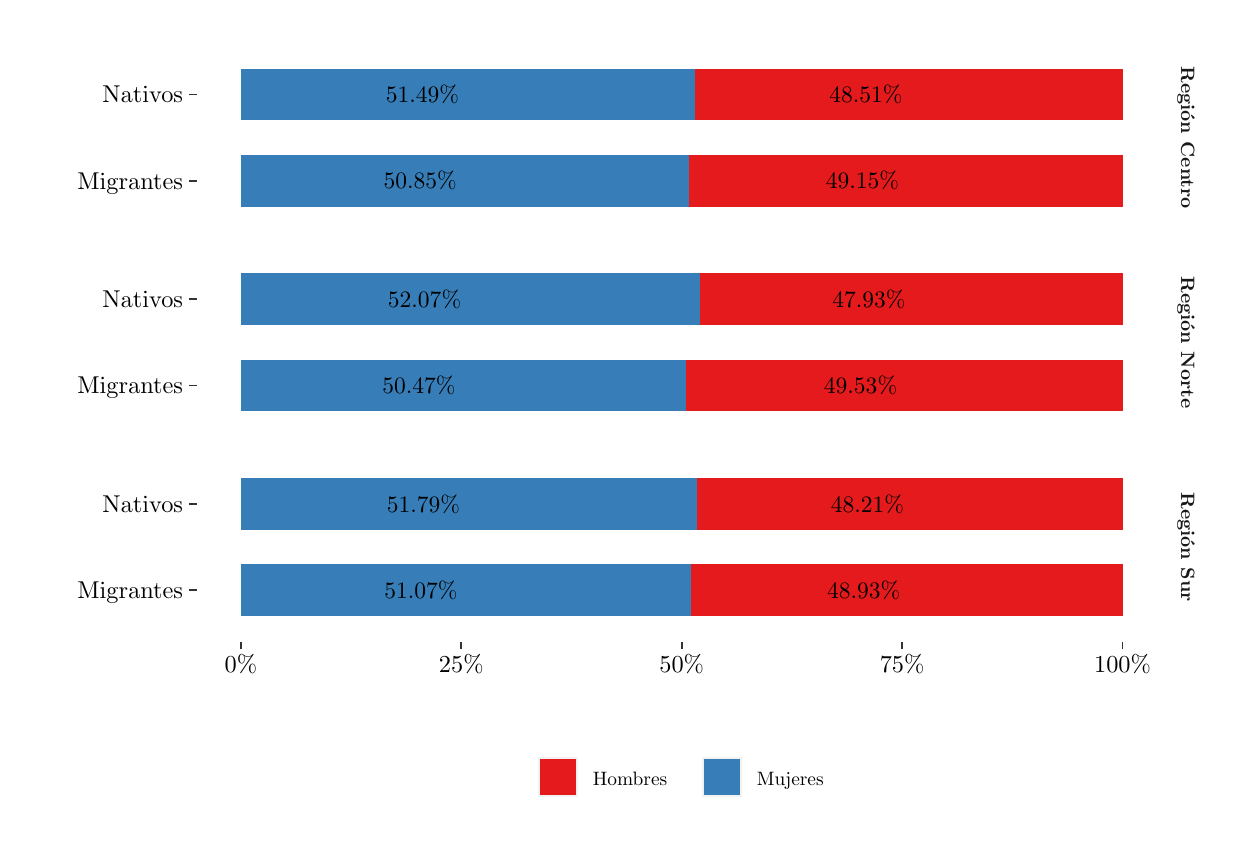
\begin{tikzpicture}[x=1pt,y=1pt]
\definecolor{fillColor}{RGB}{255,255,255}
\path[use as bounding box,fill=fillColor,fill opacity=0.00] (0,0) rectangle (433.62,289.08);
\begin{scope}
\path[clip] (  0.00,  0.00) rectangle (433.62,289.08);
\definecolor{drawColor}{RGB}{255,255,255}
\definecolor{fillColor}{RGB}{255,255,255}

\path[draw=drawColor,line width= 0.6pt,line join=round,line cap=round,fill=fillColor] (  0.00,  0.00) rectangle (433.62,289.08);
\end{scope}
\begin{scope}
\path[clip] ( 61.11,215.10) rectangle (411.55,283.58);
\definecolor{drawColor}{RGB}{255,255,255}

\path[draw=drawColor,line width= 0.3pt,line join=round] (116.86,215.10) --
	(116.86,283.58);

\path[draw=drawColor,line width= 0.3pt,line join=round] (196.51,215.10) --
	(196.51,283.58);

\path[draw=drawColor,line width= 0.3pt,line join=round] (276.15,215.10) --
	(276.15,283.58);

\path[draw=drawColor,line width= 0.3pt,line join=round] (355.80,215.10) --
	(355.80,283.58);

\path[draw=drawColor,line width= 0.6pt,line join=round] ( 61.11,233.78) --
	(411.55,233.78);

\path[draw=drawColor,line width= 0.6pt,line join=round] ( 61.11,264.90) --
	(411.55,264.90);

\path[draw=drawColor,line width= 0.6pt,line join=round] ( 77.04,215.10) --
	( 77.04,283.58);

\path[draw=drawColor,line width= 0.6pt,line join=round] (156.69,215.10) --
	(156.69,283.58);

\path[draw=drawColor,line width= 0.6pt,line join=round] (236.33,215.10) --
	(236.33,283.58);

\path[draw=drawColor,line width= 0.6pt,line join=round] (315.97,215.10) --
	(315.97,283.58);

\path[draw=drawColor,line width= 0.6pt,line join=round] (395.62,215.10) --
	(395.62,283.58);
\definecolor{fillColor}{RGB}{228,26,28}

\path[fill=fillColor] (239.03,224.44) rectangle (395.62,243.11);
\definecolor{fillColor}{RGB}{55,126,184}

\path[fill=fillColor] ( 77.04,224.44) rectangle (239.03,243.11);
\definecolor{fillColor}{RGB}{228,26,28}

\path[fill=fillColor] (241.07,255.57) rectangle (395.62,274.24);
\definecolor{fillColor}{RGB}{55,126,184}

\path[fill=fillColor] ( 77.04,255.57) rectangle (241.07,274.24);
\definecolor{drawColor}{RGB}{0,0,0}

\node[text=drawColor,anchor=base,inner sep=0pt, outer sep=0pt, scale=  0.85] at (301.66,230.84) {49.15{\%}};

\node[text=drawColor,anchor=base,inner sep=0pt, outer sep=0pt, scale=  0.85] at (141.84,230.84) {50.85{\%}};

\node[text=drawColor,anchor=base,inner sep=0pt, outer sep=0pt, scale=  0.85] at (302.89,261.96) {48.51{\%}};

\node[text=drawColor,anchor=base,inner sep=0pt, outer sep=0pt, scale=  0.85] at (142.65,261.96) {51.49{\%}};
\end{scope}
\begin{scope}
\path[clip] ( 61.11,141.12) rectangle (411.55,209.60);
\definecolor{drawColor}{RGB}{255,255,255}

\path[draw=drawColor,line width= 0.3pt,line join=round] (116.86,141.12) --
	(116.86,209.60);

\path[draw=drawColor,line width= 0.3pt,line join=round] (196.51,141.12) --
	(196.51,209.60);

\path[draw=drawColor,line width= 0.3pt,line join=round] (276.15,141.12) --
	(276.15,209.60);

\path[draw=drawColor,line width= 0.3pt,line join=round] (355.80,141.12) --
	(355.80,209.60);

\path[draw=drawColor,line width= 0.6pt,line join=round] ( 61.11,159.80) --
	(411.55,159.80);

\path[draw=drawColor,line width= 0.6pt,line join=round] ( 61.11,190.92) --
	(411.55,190.92);

\path[draw=drawColor,line width= 0.6pt,line join=round] ( 77.04,141.12) --
	( 77.04,209.60);

\path[draw=drawColor,line width= 0.6pt,line join=round] (156.69,141.12) --
	(156.69,209.60);

\path[draw=drawColor,line width= 0.6pt,line join=round] (236.33,141.12) --
	(236.33,209.60);

\path[draw=drawColor,line width= 0.6pt,line join=round] (315.97,141.12) --
	(315.97,209.60);

\path[draw=drawColor,line width= 0.6pt,line join=round] (395.62,141.12) --
	(395.62,209.60);
\definecolor{fillColor}{RGB}{228,26,28}

\path[fill=fillColor] (237.84,150.46) rectangle (395.62,169.13);
\definecolor{fillColor}{RGB}{55,126,184}

\path[fill=fillColor] ( 77.04,150.46) rectangle (237.84,169.13);
\definecolor{fillColor}{RGB}{228,26,28}

\path[fill=fillColor] (242.93,181.59) rectangle (395.62,200.26);
\definecolor{fillColor}{RGB}{55,126,184}

\path[fill=fillColor] ( 77.04,181.59) rectangle (242.93,200.26);
\definecolor{drawColor}{RGB}{0,0,0}

\node[text=drawColor,anchor=base,inner sep=0pt, outer sep=0pt, scale=  0.85] at (300.95,156.86) {49.53{\%}};

\node[text=drawColor,anchor=base,inner sep=0pt, outer sep=0pt, scale=  0.85] at (141.36,156.86) {50.47{\%}};

\node[text=drawColor,anchor=base,inner sep=0pt, outer sep=0pt, scale=  0.85] at (304.01,187.98) {47.93{\%}};

\node[text=drawColor,anchor=base,inner sep=0pt, outer sep=0pt, scale=  0.85] at (143.40,187.98) {52.07{\%}};
\end{scope}
\begin{scope}
\path[clip] ( 61.11, 67.14) rectangle (411.55,135.62);
\definecolor{drawColor}{RGB}{255,255,255}

\path[draw=drawColor,line width= 0.3pt,line join=round] (116.86, 67.14) --
	(116.86,135.62);

\path[draw=drawColor,line width= 0.3pt,line join=round] (196.51, 67.14) --
	(196.51,135.62);

\path[draw=drawColor,line width= 0.3pt,line join=round] (276.15, 67.14) --
	(276.15,135.62);

\path[draw=drawColor,line width= 0.3pt,line join=round] (355.80, 67.14) --
	(355.80,135.62);

\path[draw=drawColor,line width= 0.6pt,line join=round] ( 61.11, 85.82) --
	(411.55, 85.82);

\path[draw=drawColor,line width= 0.6pt,line join=round] ( 61.11,116.94) --
	(411.55,116.94);

\path[draw=drawColor,line width= 0.6pt,line join=round] ( 77.04, 67.14) --
	( 77.04,135.62);

\path[draw=drawColor,line width= 0.6pt,line join=round] (156.69, 67.14) --
	(156.69,135.62);

\path[draw=drawColor,line width= 0.6pt,line join=round] (236.33, 67.14) --
	(236.33,135.62);

\path[draw=drawColor,line width= 0.6pt,line join=round] (315.97, 67.14) --
	(315.97,135.62);

\path[draw=drawColor,line width= 0.6pt,line join=round] (395.62, 67.14) --
	(395.62,135.62);
\definecolor{fillColor}{RGB}{228,26,28}

\path[fill=fillColor] (239.74, 76.48) rectangle (395.62, 95.15);
\definecolor{fillColor}{RGB}{55,126,184}

\path[fill=fillColor] ( 77.04, 76.48) rectangle (239.74, 95.15);
\definecolor{fillColor}{RGB}{228,26,28}

\path[fill=fillColor] (242.02,107.61) rectangle (395.62,126.28);
\definecolor{fillColor}{RGB}{55,126,184}

\path[fill=fillColor] ( 77.04,107.61) rectangle (242.02,126.28);
\definecolor{drawColor}{RGB}{0,0,0}

\node[text=drawColor,anchor=base,inner sep=0pt, outer sep=0pt, scale=  0.85] at (302.09, 82.88) {48.93{\%}};

\node[text=drawColor,anchor=base,inner sep=0pt, outer sep=0pt, scale=  0.85] at (142.12, 82.88) {51.07{\%}};

\node[text=drawColor,anchor=base,inner sep=0pt, outer sep=0pt, scale=  0.85] at (303.46,114.00) {48.21{\%}};

\node[text=drawColor,anchor=base,inner sep=0pt, outer sep=0pt, scale=  0.85] at (143.03,114.00) {51.79{\%}};
\end{scope}
\begin{scope}
\path[clip] (411.55,215.10) rectangle (428.12,283.58);
\definecolor{drawColor}{gray}{0.10}

\node[text=drawColor,rotate=-90.00,anchor=base,inner sep=0pt, outer sep=0pt, scale=  0.70] at (416.80,249.34) {\textbf{Región Centro}};
\end{scope}
\begin{scope}
\path[clip] (411.55,141.12) rectangle (428.12,209.60);
\definecolor{drawColor}{gray}{0.10}

\node[text=drawColor,rotate=-90.00,anchor=base,inner sep=0pt, outer sep=0pt, scale=  0.70] at (416.80,175.36) {\textbf{Región Norte}};
\end{scope}
\begin{scope}
\path[clip] (411.55, 67.14) rectangle (428.12,135.62);
\definecolor{drawColor}{gray}{0.10}

\node[text=drawColor,rotate=-90.00,anchor=base,inner sep=0pt, outer sep=0pt, scale=  0.70] at (416.80,101.38) {\textbf{Región Sur}};
\end{scope}
\begin{scope}
\path[clip] (  0.00,  0.00) rectangle (433.62,289.08);
\definecolor{drawColor}{gray}{0.20}

\path[draw=drawColor,line width= 0.6pt,line join=round] ( 77.04, 64.39) --
	( 77.04, 67.14);

\path[draw=drawColor,line width= 0.6pt,line join=round] (156.69, 64.39) --
	(156.69, 67.14);

\path[draw=drawColor,line width= 0.6pt,line join=round] (236.33, 64.39) --
	(236.33, 67.14);

\path[draw=drawColor,line width= 0.6pt,line join=round] (315.97, 64.39) --
	(315.97, 67.14);

\path[draw=drawColor,line width= 0.6pt,line join=round] (395.62, 64.39) --
	(395.62, 67.14);
\end{scope}
\begin{scope}
\path[clip] (  0.00,  0.00) rectangle (433.62,289.08);
\definecolor{drawColor}{RGB}{0,0,0}

\node[text=drawColor,anchor=base,inner sep=0pt, outer sep=0pt, scale=  0.88] at ( 77.04, 56.13) {0{\%}};

\node[text=drawColor,anchor=base,inner sep=0pt, outer sep=0pt, scale=  0.88] at (156.69, 56.13) {25{\%}};

\node[text=drawColor,anchor=base,inner sep=0pt, outer sep=0pt, scale=  0.88] at (236.33, 56.13) {50{\%}};

\node[text=drawColor,anchor=base,inner sep=0pt, outer sep=0pt, scale=  0.88] at (315.97, 56.13) {75{\%}};

\node[text=drawColor,anchor=base,inner sep=0pt, outer sep=0pt, scale=  0.88] at (395.62, 56.13) {100{\%}};
\end{scope}
\begin{scope}
\path[clip] (  0.00,  0.00) rectangle (433.62,289.08);
\definecolor{drawColor}{RGB}{0,0,0}

\node[text=drawColor,anchor=base east,inner sep=0pt, outer sep=0pt, scale=  0.88] at ( 56.16,230.75) {Migrantes};

\node[text=drawColor,anchor=base east,inner sep=0pt, outer sep=0pt, scale=  0.88] at ( 56.16,261.87) {Nativos};
\end{scope}
\begin{scope}
\path[clip] (  0.00,  0.00) rectangle (433.62,289.08);
\definecolor{drawColor}{gray}{0.20}

\path[draw=drawColor,line width= 0.6pt,line join=round] ( 58.36,233.78) --
	( 61.11,233.78);

\path[draw=drawColor,line width= 0.6pt,line join=round] ( 58.36,264.90) --
	( 61.11,264.90);
\end{scope}
\begin{scope}
\path[clip] (  0.00,  0.00) rectangle (433.62,289.08);
\definecolor{drawColor}{RGB}{0,0,0}

\node[text=drawColor,anchor=base east,inner sep=0pt, outer sep=0pt, scale=  0.88] at ( 56.16,156.77) {Migrantes};

\node[text=drawColor,anchor=base east,inner sep=0pt, outer sep=0pt, scale=  0.88] at ( 56.16,187.89) {Nativos};
\end{scope}
\begin{scope}
\path[clip] (  0.00,  0.00) rectangle (433.62,289.08);
\definecolor{drawColor}{gray}{0.20}

\path[draw=drawColor,line width= 0.6pt,line join=round] ( 58.36,159.80) --
	( 61.11,159.80);

\path[draw=drawColor,line width= 0.6pt,line join=round] ( 58.36,190.92) --
	( 61.11,190.92);
\end{scope}
\begin{scope}
\path[clip] (  0.00,  0.00) rectangle (433.62,289.08);
\definecolor{drawColor}{RGB}{0,0,0}

\node[text=drawColor,anchor=base east,inner sep=0pt, outer sep=0pt, scale=  0.88] at ( 56.16, 82.79) {Migrantes};

\node[text=drawColor,anchor=base east,inner sep=0pt, outer sep=0pt, scale=  0.88] at ( 56.16,113.91) {Nativos};
\end{scope}
\begin{scope}
\path[clip] (  0.00,  0.00) rectangle (433.62,289.08);
\definecolor{drawColor}{gray}{0.20}

\path[draw=drawColor,line width= 0.6pt,line join=round] ( 58.36, 85.82) --
	( 61.11, 85.82);

\path[draw=drawColor,line width= 0.6pt,line join=round] ( 58.36,116.94) --
	( 61.11,116.94);
\end{scope}
\begin{scope}
\path[clip] (  0.00,  0.00) rectangle (433.62,289.08);
\definecolor{fillColor}{RGB}{255,255,255}

\path[fill=fillColor] (173.29,  5.50) rectangle (299.37, 30.95);
\end{scope}
\begin{scope}
\path[clip] (  0.00,  0.00) rectangle (433.62,289.08);
\definecolor{fillColor}{gray}{0.95}

\path[fill=fillColor] (184.29, 11.00) rectangle (198.74, 25.45);
\end{scope}
\begin{scope}
\path[clip] (  0.00,  0.00) rectangle (433.62,289.08);
\definecolor{fillColor}{RGB}{228,26,28}

\path[fill=fillColor] (185.00, 11.71) rectangle (198.03, 24.74);
\end{scope}
\begin{scope}
\path[clip] (  0.00,  0.00) rectangle (433.62,289.08);
\definecolor{fillColor}{gray}{0.95}

\path[fill=fillColor] (243.54, 11.00) rectangle (257.99, 25.45);
\end{scope}
\begin{scope}
\path[clip] (  0.00,  0.00) rectangle (433.62,289.08);
\definecolor{fillColor}{RGB}{55,126,184}

\path[fill=fillColor] (244.25, 11.71) rectangle (257.28, 24.74);
\end{scope}
\begin{scope}
\path[clip] (  0.00,  0.00) rectangle (433.62,289.08);
\definecolor{drawColor}{RGB}{0,0,0}

\node[text=drawColor,anchor=base west,inner sep=0pt, outer sep=0pt, scale=  0.70] at (204.24, 15.20) {Hombres};
\end{scope}
\begin{scope}
\path[clip] (  0.00,  0.00) rectangle (433.62,289.08);
\definecolor{drawColor}{RGB}{0,0,0}

\node[text=drawColor,anchor=base west,inner sep=0pt, outer sep=0pt, scale=  0.70] at (263.49, 15.20) {Mujeres};
\end{scope}
\end{tikzpicture}
